%% Desarrollo PSO velocidad

\chapter{PSO para la dirección del viento en Valparaíso}
\section{Modelo Matemático}\label{ss:model_math_dir} 
Como se comenta anteriormente, la distribución de densidad de probabilidad que se utilizará para describir la distribución de datos de dirección del viento
es la \emph{finite mixtures of von mises distribution} descrita en \ref{eq:mixtureVonMises}, la cual consiste básicamente en una combinación lineal de la \emph{simple von Mises distribution} descrita en \ref{eq:simpleVonMises}.\\ 
De forma preliminar, los datos se ordenan en un histograma de densidad con el cual se obtiene un esqueleto de la distribución de densidad de probabilidad. Posteriormente se requieren encontrar los parámetros de ajuste $\mu_j$, $k_j$ y $w_j$ para cada $j$-ésima \emph{simple von Mises distribution}. La forma en que
se realiza esto último en este trabajo está basado en el documento de Carta et al. \cite{Carta07} y se describe a continuación.\\
Para la construcción del histograma se divide el rango de datos que va de 0 a $2\pi$ en $T$ clases con frecuencia $O_i$ la cual representa la suma de las observaciones en el rango de la clase $T$. Posteriormente se definen $k$ sectores del mismo largo desde las $T$ clases, relacionados al número de direcciones de viento predominantes (o con mayor frecuencia). Esto define el número de funciones de von Mises a utilizar. La estimación de $k$ se realiza mediante la observación del histograma de los datos, observando la cantidad de direcciones con altas frecuencias (también puede ser considerado un parámetro de ajuste, que requiera de pruebas empíricas para encontrar el valor adecuado). Además, se sigue la observación empírica en el trabajo de Carta et al. \cite{Carta07}, en donde se concluye que valores superiores a 6 \emph{mixtures} no mejoran considerablemente la calidad del ajuste.\\
Para la aproximación inicial de los parámetros de la \emph{mixture of von mises distribution} se utiliza una estimación numérica, utilizada por Heckenbergerova et al. \cite{Heckenbergerova15} \cite{Heckenbergerova13} y Carta et al. \cite{Carta07}, basada en los datos recolectados acerca de la dirección del viento.\\
Sea $j \in \{1 ... k\}$ el subíndice del sector representado por la $j$-ésima función de von Mises.\\
La dirección del viento predominante $\mu_j$ se estima de la siguiente forma:
\begin{align}\label{eq:Prevailing_Param}
    \mu_j &= 
        \left\{
            \begin{array}{ll}
                arctan(\frac{s_j}{c_j})  & s_j \geq 0, c_j > 0\\
                \frac{\pi}{2} & s_j > 0, c_j = 0\\
                \pi + arctan(\frac{s_j}{c_j}) & c_j < 0\\
                \pi & s_j > 0, c_j = -1\\
                2\pi + arctan(\frac{s_j}{c_j}) & s_j < 0, c_j > 0\\
                3\frac{\pi}{2} & s_j < 0, c_j = 0\\
            \end{array}
        \right.
\end{align}
En donde $s_j$ y $c_j$ representan el seno y coseno promedio del sector $j$.\\
Tradicionalmente, se estima el parámetro de concentración $k_j$ con la ecuación:
\begin{align}\label{eq:Implicit_Param}
    \frac{I_1(k_j)}{I_0(k_j)} = \sqrt{s_j^2 + c_j^2}
\end{align}
Donde $I_1(k_j)$ es la función modificada de Bessel de primera clase y orden 1.
 Como se explica en Banerjee et al. \cite{Banerjee05}, debido a la falta de una solución análitica a la ecuación \ref{eq:Implicit_Param}, no es posible estimar directamente los valores de $k$. Se podrían utilizar métodos para ecuaciones no lineales, pero para datos de altas dimensiones, problemas de desbordamiento (\emph{overflow}) o inestabilidad numérica se vuelven concurrentes. Por tanto, se utiliza la propuesta realizada en el trabajo de Heckenbergerova et al. \cite{Heckenbergerova15} con lo cual el parámetro $k_j$ puede ser aproximado por:\\
\begin{align}
    |k_j| = \{23.29041409 - 16.8617370\sqrt[4]{s_j^2 + c_j^2}\} 
\end{align}
También existe otra forma similar a esta aproximación, utilizada por  Heckenbergerova et al. en \cite{Heckenbergerova13} y por Carta et al. \cite{Carta07}, la cual consiste en 
la siguiente fórmula:\\
\begin{align}
    k_j = \{23.29041409 - 16.8617370\sqrt[4]{s_j^2 + c_j^2} - 17.4749884 exp(-(s_j^2 + c_j^2))\}^{-1} 
\end{align}
Los pesos iniciales $w_j$ son aproximados como: \\
\begin{align}\label{eq:Weight_Param}
    w_j = \frac{\sum_{i=J_l}^{J_u} O_i}{\sum_{i=1}^{T} O_i}
\end{align}

Donde $J_l$ y $J_u$ son los índices de los bordes del sector $j$.\\
La función objetivo para el PSO es el test estadístico $\chi^2$ descrito en Heckenbergerova et al. \cite{Heckenbergerova15} como sigue a continuación:
\begin{align}\label{eq:FO_Direction}
    \chi^2 = \sum_{i=1}^{T}\frac{(O_i - np_{i})^2}{np_i}
\end{align}
Donde $T$ es el número de clases de frecuencia definido para construir el histograma, $n$ es la suma de las frecuencias observadas $O_i$ y $p_i$ es la probabilidad teórica de cada clase de frecuencia predicha por el modelo ajustado.\\
Para el cálculo del $p_i$ se utiliza:
\begin{align}
    p_i = \int_{l_i}^{u_i} f(x) dx
\end{align}
Donde $u_i$ y $l_i$ son los bordes de la $i$-ésima clase de frecuencia.\\
La forma de la solución a encontrar es descrita en \ref{eq:sol_pso}. Esta es restringida por la condición para los pesos de la \emph{mixture von Mises distribution}, la cual obliga a que se deba cumplir que la suma de los pesos sea igual a 1, como se describe en la sección \ref{eq:WeightConstraint}.

\section{Estructura del PSO}
Es esta sección se detallará cada una de los componentes del algoritmo para el ajuste de los parámetros de la distribución de von Mises para la dirección del viento. A diferencia del algoritmo anterior, en este se incluye una estimación inicial de la solución y una propuesta al manejo de parámetros del PSO.
\subsection{Representación}\label{sec:Representacion}
La representación del PSO es similar al utilizado para el ajuste de la distribución de datos de velocidad del viento. Las partículas y el enjambre están representados por las ecuaciones descritas en \ref{rep:Particle} y \ref{rep:Swarm} respectivamente.\\
La solución para el PSO que mejora la estimación inicial de los parámetros para la \emph{mixture von Mises distribution} está representado por un vector $v$ en el cual se encuentran los valores para todos los parámetros de cada \emph{simple von Mises distribution}. Estos valores están codificados para que el algoritmo se mueve en el rango desde 0 a 1.\\
El vector solución tiene la forma:
\begin{align}
    v = (\overbrace{v_1,...,v_k}^{\mu},\overbrace{v_{k+1},...,v_{2k}}^{k},\overbrace{v_{2k+1},...,v_{n}}^{w}).
\end{align}
El parámetro $\mu$ está representado en el rango $i \in \{1,...,k\}$ y para ser decodificado debe ser escalado por $2\pi$.\\
El parámetro $k$ está representado en el rango $i \in \{k+1,...,2k\}$ y para ser decodificado debe ser escalado por $[0, 700]$.\\
El parámetro $w_j$ está representado en el rango $i \in \{2k+1,...,n\}$ cuyos valores van en el rango $[0,1]$.

\subsection{Consideración de los parámetros}\label{subsec:parametros_new}
En el trabajo de Heckenbergerova et al. \cite{Heckenbergerova15} los parámetros del PSO son fijados de la siguiente forma.
\begin{enumerate}
  \item Para el factor de inercia $w$ el valor es 0.89.
  \item Para el factor cognitivo $c_1$ el valor es 0.5.
  \item Para el factor social $c_2$ el valor es 0.7.
\end{enumerate}
Sin embargo, como se concluye en su trabajo y de acuerdo a los resultados de la tabla \ref{table:stadistical_tests_direction}, estos valores no generan resultados satisfactorios, es decir, las soluciones encontradas bajo esos parámetros, al ser evaluadas en la función objetivo, no satisfacen los requerimientos para el test realizado por ellos mismos. Por esto, en esta memoria se propone una estrategia distinta para el control de los parámetros del PSO, la cual se compara con la estrategia de parámetros fijos, a través de experimentos que utilizan ambas técnicas.\\ 
Anteriormente se menciona la estrategia sugerida en el trabajo de Chang \cite{Chang10_2} para la variación de parámetros del PSO, descrita en \ref{eq:VariationParameters}, con el fin de evitar una convergencia prematura en el ajuste de la distribución de Weibull. Esta estrategia podría ser considerada para intentar mejorar los resultados conseguidos por Heckenbergerova et al. \cite{Heckenbergerova15}, sin embargo, la sugerencia presenta inconvenientes por que depende del número de iteraciones máximo que se defina para el algoritmo.\\
Al realizarse diversas pruebas con cantidad de iteraciones distintas, se puede evidenciar que el hecho de que el número de iteraciones máximo sean un valor que afecta la variación de parámetros, tiene como consecuencia que el algoritmo tome diferentes caminos hacia la solución final, por ende, un aumento en el número de iteraciones no constituiría necesariamente una mejora en calidad de la solución. De cierta forma, el número de iteraciones máximo se transforma en un factor pseudo-aleatorio para el PSO.\\
Por lo tanto, debido a que los parámetros fijos no consiguen buenos resultados y la variación de parámetros propuesta por Chang \cite{Chang10_2} presenta inconvenientes estructurales para el PSO, se propone el siguiente método para el ajuste de parámetros.\\

\subsection{Propuesta para la variación de parámetros del PSO}
Sean $w(j)$, $c_1(j)$ y $c_2(j)$ los parámetros de inercia, cognitivo y social del PSO en el instante $j$ respectivamente:  
\begin{align}\label{eq:VariationParameters_new}
    w(j) &= w(j) + (w_{max} - w(j)) * F \\\label{eq:VariationParameters_new_2}
    c_{1}(j) &= c_1(j) + (c_{1max} - c_1(j)) * F \\\label{eq:VariationParameters_new_3}
    c_{2}(j) &= c_2(j) + (c_{2min} - c_2(j)) * F
\end{align} 
Donde $F$ es un factor de avance dentro de un rango definido para los parámetros el cual está en función de una valor de la función objetivo esperado y el valor actual de la solución. Es decir: 
\begin{align}
  F = \frac{\text{Valor esperado en la FO}}{\text{Valor actual en la FO}}
\end{align}
Si el factor $F$ sobrepasa el valor de 1 (caso en el que la solución actual es mejor que la esperada considerando la minimización de la función objetivo), se deja de cambiar los parámetros. Esto se resume como:
\begin{align}\label{eq:restriction_var_par_new}
    F &= 
        \left\{
            \begin{array}{ll}
                \frac{P}{p_j}  & P \leq p_j\\
                0 & P > p_j\\
            \end{array}
        \right.
\end{align}
Donde $P$ es un valor esperado para la función objetivo (definido como parámetro) y $p_j$ es el valor en la función objetivo de la mejor solución hasta el momento. La actualización de parámetros se realiza solamente cuando se mejora la solución global actual. La variación tiene la misma lógica que la propuesta de Chang \cite{Chang10_2}, es decir, abolir el aporte de la solución global hacia el final de las iteraciones.\\
En síntesis, el cambio de los parámetros se produce en proporción a la distancia del valor actual con respecto a un valor final y a razón de un valor esperado para la función objetivo sobre el valor actual de la mejor solución.\\
 Con esto se logra mejorar el rendimiento del algoritmo alcanzando mejores soluciones en tiempos menores de ejecución como se puede observar en la sección de resultados \ref{sec:Resultados_Dir}.

\subsection{Descripción del algoritmo}
La estructura del algoritmo definida para el PSO consiste en dos fases. La primera, una aproximación basada en la estimación numérica de los parámetros requeridos para la \emph{mixture of von Mises distribution} a través de operaciones simples con los datos recolectados, y la segunda, una mejora de la solución inicial obtenida en la fase anterior mediante el uso de la meta-heurística \emph{Particle Swarm Otimization}. \\
El método para la aproximación inicial de la solución se detalla en el Algoritmo \ref{alg:init_aprox_direction}.
En donde la estimación de los parámetros se realiza como se describe en la ecuación \ref{eq:Prevailing_Param} para los $\mu_j$, la ecuación \ref{eq:Implicit_Param} para los $k_j$ y  la ecuación \ref{eq:Weight_Param} para los pesos $w_j$.
%!TEX root = main.tex

\caption{Aproximación inicial de los parámetros de la \emph{mixture von Mises distribution}}
\begin{algorithmic}
\REQUIRE Datos de frecuencias de la dirección del viento.
\REQUIRE K, Cantidad de \emph{simple von Mises distribution}.
\REQUIRE T, clases de frecuencias.
\REQUIRE D, Total de datos.
\ENSURE Valores para los parámetros $\mu_j$, $k_j$ y $w_j$, para cada $j \in \{1,...,k\}$.
\STATE sol = inicializarVectorSolución(3*K)
\FOR{$j = 0$ to $K$}

\STATE datos$_j$ = datosEnRango($j*D/K$)
\STATE s$_j$ = obtenerSenoPromedio(datos$_j$)
\STATE c$_j$ = obtenerCosenoPromedio(datos$_j$)
\STATE u$_j$ = obtenerDirecciónPredominante(s$_j$,c$_j$)
\STATE k$_j$ = obtenerConcentración(s$_j$, c$_j$)
\STATE w$_j$ = obtenerPeso($j*(T/K)$, $(j + 1)*(T/K)$)
\STATE addToSolution(sol, u$_j$, k$_j$, w$_j$)

\ENDFOR
\STATE retornarSoluciónInicial(sol).
\end{algorithmic}
Una vez obtenida la aproximación inicial se procede a mejorar esta mediante el uso del PSO descrito en el Algoritmo \ref{alg:pso_direction}.
%!TEX root = main.tex
\caption{PSO para la mejora de la aproximación de los parámetros de la \emph{mixture von Mises distribution}}
\begin{algorithmic}
\REQUIRE Datos de la dirección del viento.
\REQUIRE Solución inicial para el ajuste de la \emph{mixture von Mises distribution}.
\ENSURE Solución inicial mejorada.
\STATE enjambre = inicializar(w,c1,c2)
\FOR{$i = 1$ to $Iter_{max}$}
\FOR{Each partículas en enjambre}
    \STATE actualizarVelocidadPartícula(partícula)
    \STATE actualizarPosiciónPartícula(partítcula)
    \STATE revisarLímitesPosición(partícula)
    \STATE guardarMejorResultadoPartícula(partícula)
\ENDFOR
\STATE guardarMejorResultadoGlobal(enjambre)
\STATE actualizarParámetros(enjambre)
\ENDFOR
\STATE retornarMejorResultadoGlobal(enjambre).
\end{algorithmic}
Para la inicialización de las partículas, se realizaron pequeñas perturbaciones a la solución inicial tal y como se sugiere en Heckenbergerova et al. \cite{Heckenbergerova15}. Esto evita que la solución escape a zonas que tengan un buen resultado en la función objetivo, pero cuya forma escape a la del histograma. Debido a que la función objetivo definida en \ref{eq:FO_Direction} mide las diferencias de frecuencias entre los datos reales y los teóricos, es decir, las áreas de las barras del histograma de densidad versus el área bajo la curva de la distribución de probabilidad en algún intervalo, más de una forma de la curva podría parecer una buena solución como se vé en el gráfico de mal ajuste \ref{fig:pso_valpo_15_14_13_lq}. Por ello, la idea es mantener la forma inicial encontrada, mejorándola sin deformarla. Así, las perturbaciones iniciales a los valores de las posiciones de las partículas eran del orden de $~ 10^{-3}$.\\
Los parámetros del PSO varían de acuerdo a lo definido anteriormente en las ecuaciones \ref{eq:VariationParameters_new}, \ref{eq:VariationParameters_new_2} y \ref{eq:VariationParameters_new_3}.\\
La forma en que se cuidaron las condiciones de borde consistieron en limitar el avance de las partículas a los bordes 0 y 1 manteniéndolos en dichos valores si es que se excedían a ellos.\\
Para cuidar la restricción de pesos se normalizaran los valores determinados en cada iteración, es decir, se suman todos los valores $w_j$ y se ponderan dichos valores por el recíproco de la suma obtenida.\\
Debido a que la función objetivo implica determinar la frecuencia teórica, es necesario determinar la probabilidad
de cierto rango de direcciones mediante el cálculo del área bajo la curva de la distribución de densidad de probabilidad, para luego multiplicarla por la suma del total de datos y así obtener el valor requerido. Por ende, para el cálculo de la integral se utilizaron sumas de Riemann con una partición conveniente al desempeño del algoritmo y la precisión requerida.\\
Finalmente, la solución obtenida es decodificada tal y como se explica en la sección \ref{sec:Representacion}.\\

\section{Resultados}\label{sec:Resultados_Dir}
En esta sección se presentan los experimentos realizados y los resultados obtenidos al realizar el ajuste de los parámetros de la \emph{mixture of von Mises distribution} a los datos de dirección del viento mediante el uso del PSO.
\subsection{Experimentos}
Similar a los descrito en la sección \ref{sec:Experimentos_velocidad}, los datos de dirección del viento son tratados para rescatar las mediciones pertinentes al trabajo aquí expuesto. Estos se encuentran inicialmente en un formato como el que se puede apreciar en la Figura \ref{fig:example_data}.\\
Nuevamente, las pruebas fueron realizadas en un computador con sistema operativo Ubuntu 16.04 64-bit, 3.8 GB de memoria y procesador doble núcleo Intel Pentium 2.60 GHz.\\
Para evaluar la calidad de la solución, se utilizó el test de Chi cuadrado (\emph{Chi square goodness fit})\cite{goodFitTest}, con lo cual se evalúa qué tan bien representa el modelo propuesto a los datos medidos. Para ello, la hipótesis nula $H_0$ afirma que los datos de dirección del viento se distribuyen según la función de densidad \emph{mixture of von Mises distribution} y la hipótesis alternativa $H_1$ niega dicha afirmación. Se rechaza $H_0$ si el valor de la función objetivo del PSO para la solución final encontrada excede el valor crítico de $\chi^2$ para un nivel de significancia de $\alpha = 0.05$ y 13 grados de libertad, es decir \textbf{22.362}, valor que puede encontrarse en la tabla de la distribución $\chi^2$ \cite{chiSquareTable}. Los grados de libertad son definidos a partir de la cantidad de clases de frecuencia definidas para el estudio, en este caso, se dividió el rango de valores de $[0, 2\pi]$ en 14 tramos iguales, por lo que quedan $(n-1)$ grados de libertad, 13 en este caso.\\
Los experimentos consistieron en el ajuste de varios subconjuntos de datos provenientes de las mediciones obtenidas para la dirección del viento en los años 2013, 2014 y 2015. Así, se prueba la utilidad de la propuesta realizada independiente del rango de tiempo a modelar.\\
Es importante considerar que no se incluyen los días en los que no hubo viento por la evidente imposibilidad de registrar la dirección.
Los subconjuntos definidos fueron los siguientes:
\begin{enumerate}
    \item \textbf{Anual}: Se consideran los datos de todo el año elegido (2013, 2014, 2015).
    \item \textbf{Meses acumulados}: Se considera una agrupación mensual pero reuniendo los datos de tres años consecutivos (2013, 2014, 2015). Es decir, para el mes de Enero, se ajusta el modelo a los datos de Enero-2013, Enero-2014 y Enero-2015 en conjunto.
    \item \textbf{Meses}: Se escogen algunos meses para ser comparados consigo mismos durante los tres años escogidos. Por ejemplo, Enero-2013, Enero-2014 y Enero-2015 por separado.       
\end{enumerate}

Para el funcionamiento del PSO, se estableció un límite de 50500 iteraciones, se utilizaron 100 partículas, y se usó como criterio de parada si es que el valor en la función objetivo de la mejor solución encontrada al momento era menor a 22.362 (criterio basado en la estrategia de cumplir el test \emph{Chi square goodness fit}). El mismo valor se estableció como valor esperado para la función objetivo al utilizarse la variación de parámetros definida en las ecuaciones \ref{eq:VariationParameters_new},  \ref{eq:VariationParameters_new_2} y \ref{eq:VariationParameters_new_3}. Además, se estableció un límite de tiempo de 30 minutos de ejecución por experimento.\\
La cantidad de \emph{mixture of simple von Mises distribution} utilizadas fue de 7, siguiendo la recomendación de Carta et al. \cite{Carta07} y algunas pruebas iniciales.\\
Con el fin de evitar que los resultados estén sesgados por el azar, dado los factores aleatorios presentes en la fórmula del PSO 
\ref{rep:Swarm}, se repiten los experimentos realizados 30 veces cambiando la semilla generadora de números aleatorios.\\

Por último, se comparan los resultados obtenidos por el PSO propuesto en el trabajo de Heckenbergerova et al. \cite{Heckenbergerova15} con la propuesta realizada en esta memoria para la variación de parámetros del PSO definidas en las ecuaciones \ref{eq:VariationParameters_new}, \ref{eq:VariationParameters_new_2} y \ref{eq:VariationParameters_new_3}.

\subsection{Análisis de los resultados}
\subsubsection{Experimento 1, pruebas iniciales}

En la Figura \ref{fig:BAD_ADJUST} se puede observar un ajuste bastante distorsionado respecto al histograma de datos. Esto se debe a que la función objetivo del PSO evalúa la diferencia entre las frecuencias experimentales y las obtenidas teóricamente, por lo tanto, diferentes curvas pueden tener igual magnitud del área bajo la curva y por ende, la misma probabilidad con la que se obtiene la frecuencia teórica.\\
Por esto, es importante que el PSO busque mejorar la solución inicial en una vecindad cercana a esta, de manera de obtener una evolución como la que se aprecia en la Figura \ref{fig:EV_SOL}. Para lograr esto, el algoritmo debe inicializar las partículas en la posición de la solución inicial encontrada más una pequeña perturbación.   
\begin{figure}[ht!]
     \centering
     \captionsetup{justification=centering,margin=2cm}
        \subfigure[Ejemplo de mal ajuste, 2015.]{
            \label{fig:BAD_ADJUST}
            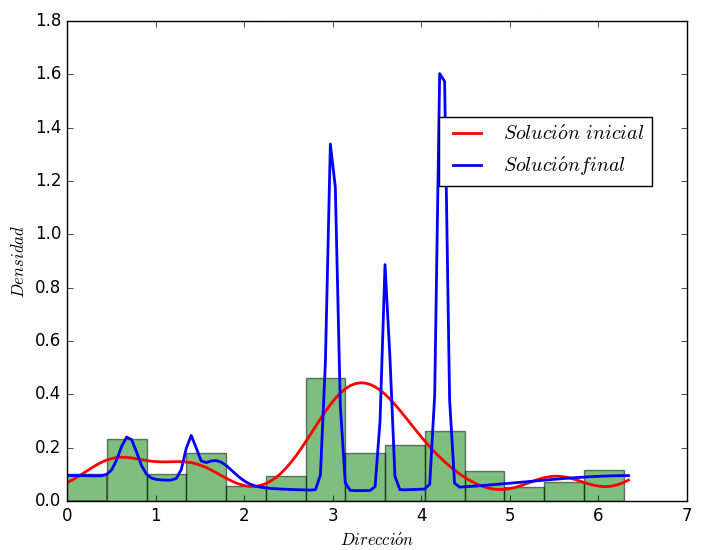
\includegraphics[width=0.45\textwidth]{figures/bad_adjust.png}
        }
        \subfigure[Evolucion de la solución.]{
            \label{fig:EV_SOL}
            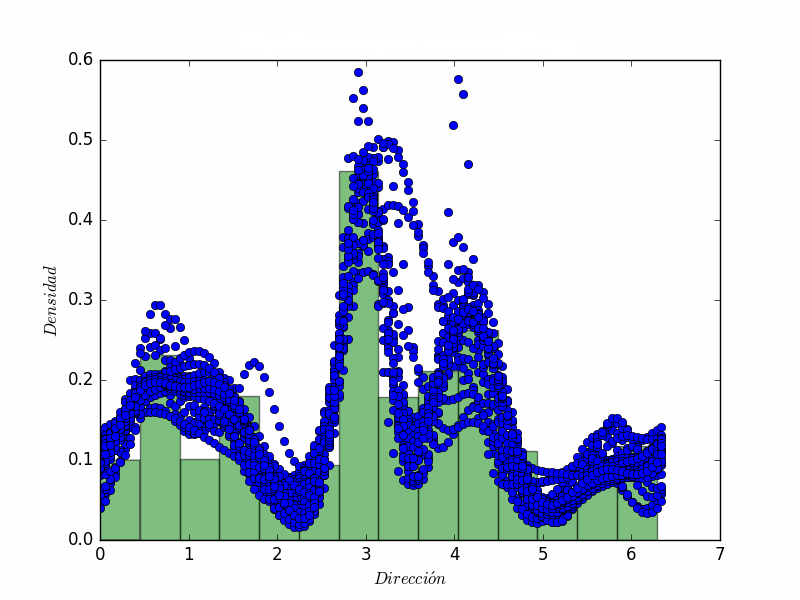
\includegraphics[width=0.45\textwidth]{figures/ev_solution.png}
        }%
    \caption{Pruebas iniciales.}
    \caption*{Fuente: Elaboración propia.}
    \label{fig:subfigures}
\end{figure}

\subsubsection{Experimento 2, Ajustes anuales}
En este experimento se ajustan los vientos anualmente, en los años de los cuales se obtuvieron datos para este estudio, resultado la Figura \ref{fig:SOL_13} para el 2013, la Figura \ref{fig:SOL_14} para el 2014 y la Figura \ref{fig:SOL_15} para el 2015.
Tal como se realiza en otros estudios \cite{Heckenbergerova15} \cite{Winddirelse15}, el ajuste de los datos de dirección del viento en un formato
de largo plazo, permite observar el comportamiento global de los vientos pudiendo evaluar la norma o generalidad en los datos registrados.
En las Figuras referenciadas previamente se observa la evolución de la solución desde la aproximación inicial hasta la mejorada por el PSO.

\begin{figure}[ht!]
     \centering
     \captionsetup{justification=centering,margin=2cm}
        \subfigure[Solución inicial y final, 2015.]{
           \label{fig:SOL_15}
           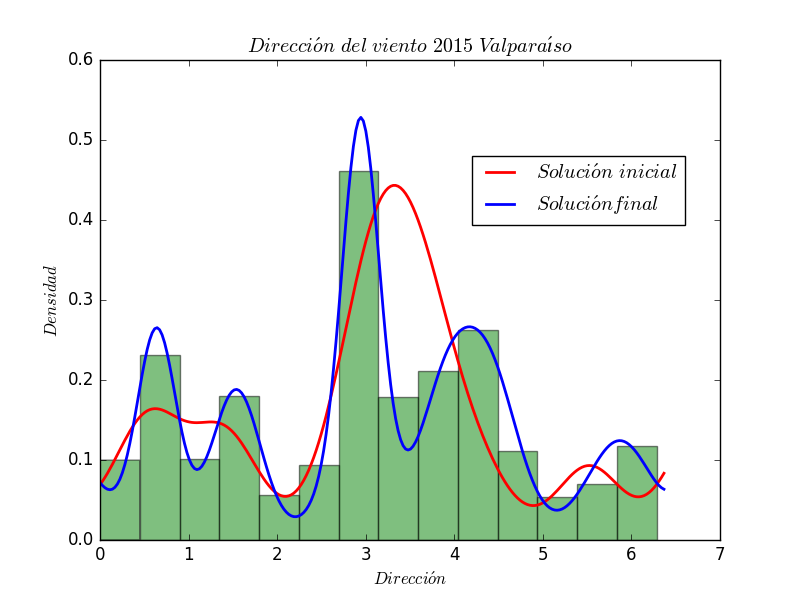
\includegraphics[width=0.45\textwidth]{figures/sol_ini_sol_fin.png}
        }
        \subfigure[Solución inicial y final, 2014.]{
            \label{fig:SOL_14}
            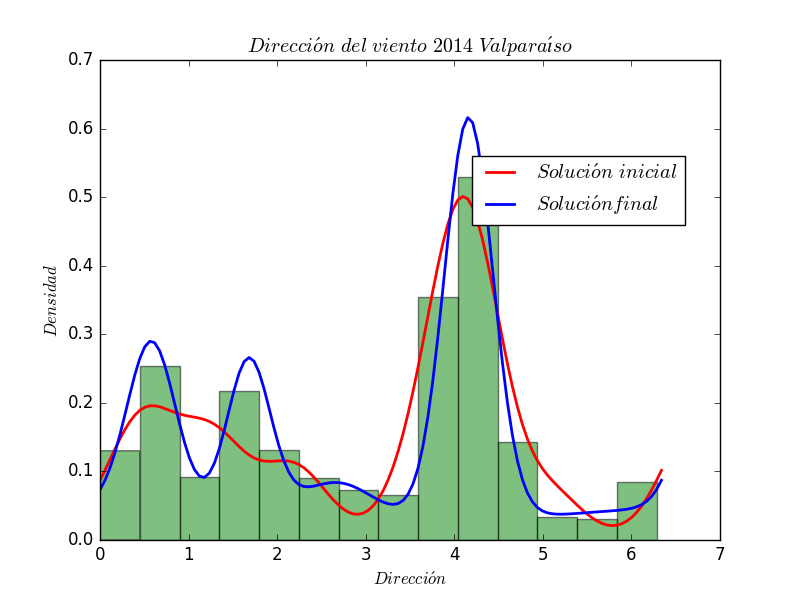
\includegraphics[width=0.45\textwidth]{figures/sol_ini_sol_fin_2014.png}
        }\\
         \subfigure[Solución inicial y final, 2013.]{
            \label{fig:SOL_13}
            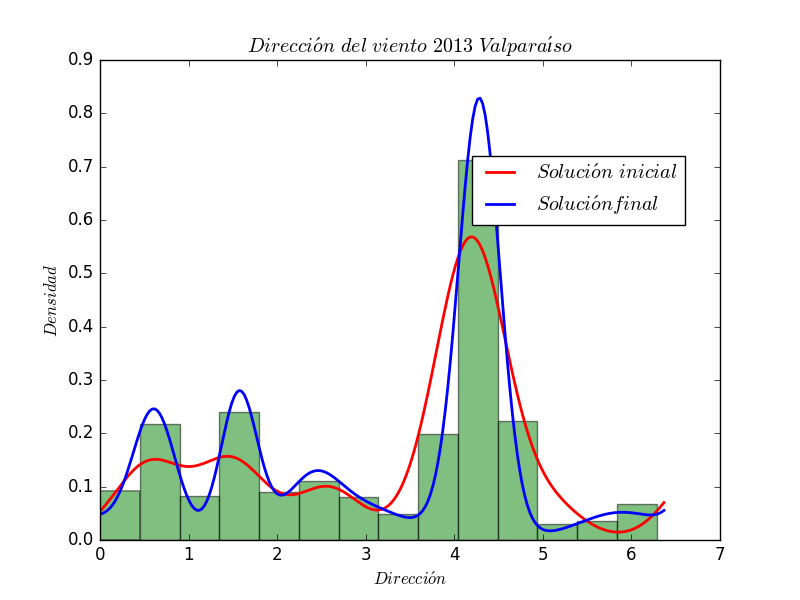
\includegraphics[width=0.45\textwidth]{figures/sol_ini_sol_fin_2013.png}
        }
    \caption{Graficos de ajustes anuales.}
    \caption*{Fuente: Elaboración propia.}
    \label{fig:subfigures}
\end{figure}

\subsubsection{Experimento 3, Ajustes de meses acumulados}
Similar al ejercicio anterior, los gráficos agrupados en \ref{fig:PLOT_MONTHS_ALL_1} y \ref{fig:PLOT_MONTHS_ALL_2}, permiten visualizar el ajuste de los datos del viento por meses. En este caso se agruparon los datos de los tres años escogidos por cada mes, es decir, la Figura \ref{fig:PLOT_SOL_ENERO}, por ejemplo, contiene los datos del mes de enero de los años 2013, 2014 y 2015.\\
Se puede observar que algunos gráficos muestran un mejor ajuste que otros, a pesar del correcto valor obtenido en la función objetivo como se expresa posteriormente en la tabla \ref{table:stadistical_tests_direction}. Esto se debe a que probablemente la solución se escapa más de los deseado de la solución inicial. 
\begin{figure}[ht!]
    \centering
    \captionsetup{justification=centering,margin=2cm}
         %%MONTHS  
        \subfigure[Solución inicial y final, Enero.]{
            \label{fig:PLOT_SOL_ENERO}
            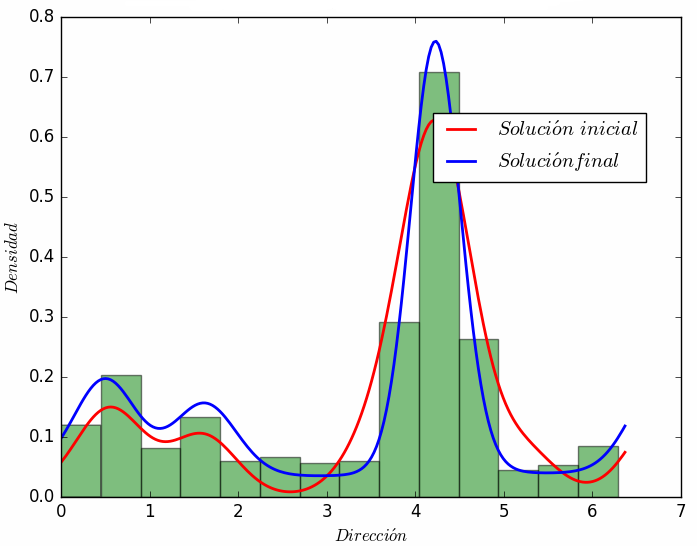
\includegraphics[width=0.42\textwidth]{figures/sol_ini_sol_fin_ENERO.png}
        }
         \subfigure[Solución inicial y final, Febrero.]{
            \label{fig:PLOT_SOL_FEBRERO}
            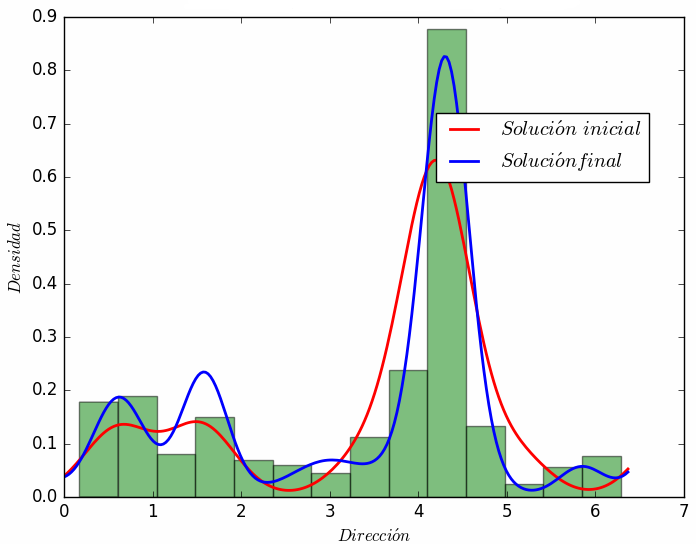
\includegraphics[width=0.42\textwidth]{figures/sol_ini_sol_fin_FEBRERO.png}
        }\\
          \subfigure[Solución inicial y final, Marzo.]{
            \label{fig:PLOT_SOL_MARZO}
            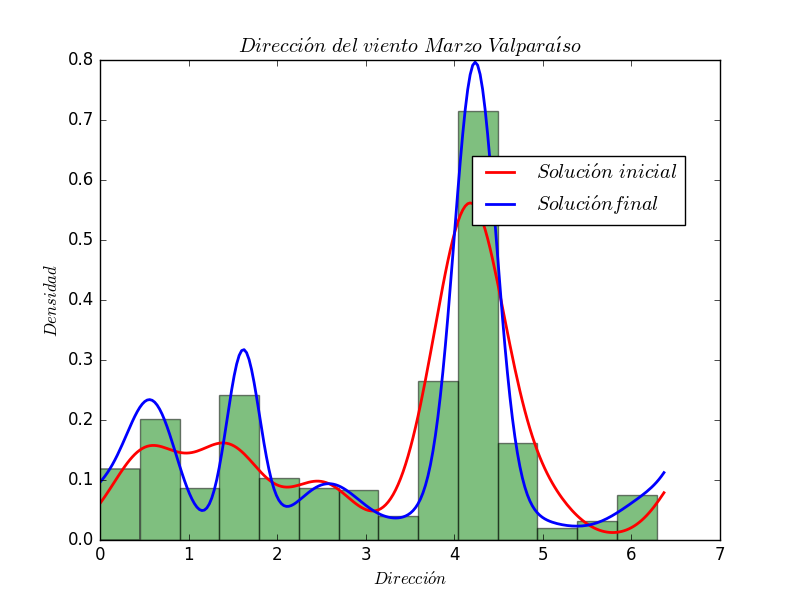
\includegraphics[width=0.42\textwidth]{figures/sol_ini_sol_fin_MARZO.png}
        }
         \subfigure[Solución inicial y final, Abril.]{
            \label{fig:PLOT_SOL_ABRIL}
            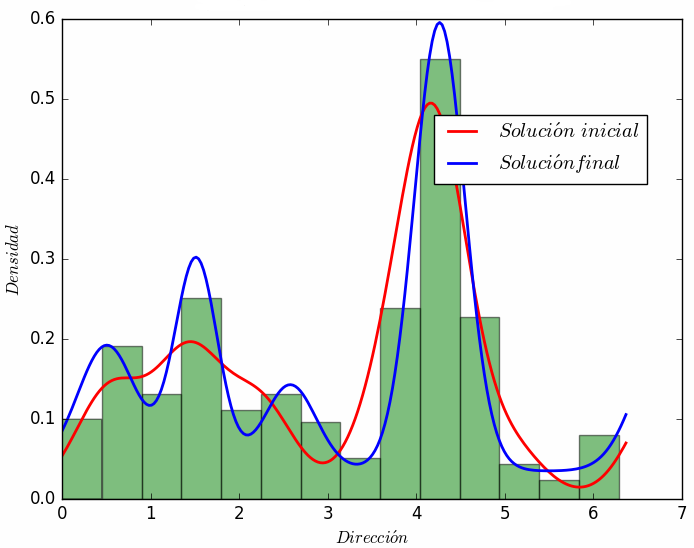
\includegraphics[width=0.42\textwidth]{figures/sol_ini_sol_fin_ABRIL.png}
        }\\
          \subfigure[Solución inicial y final, Mayo.]{
            \label{fig:PLOT_SOL_MAYO}
            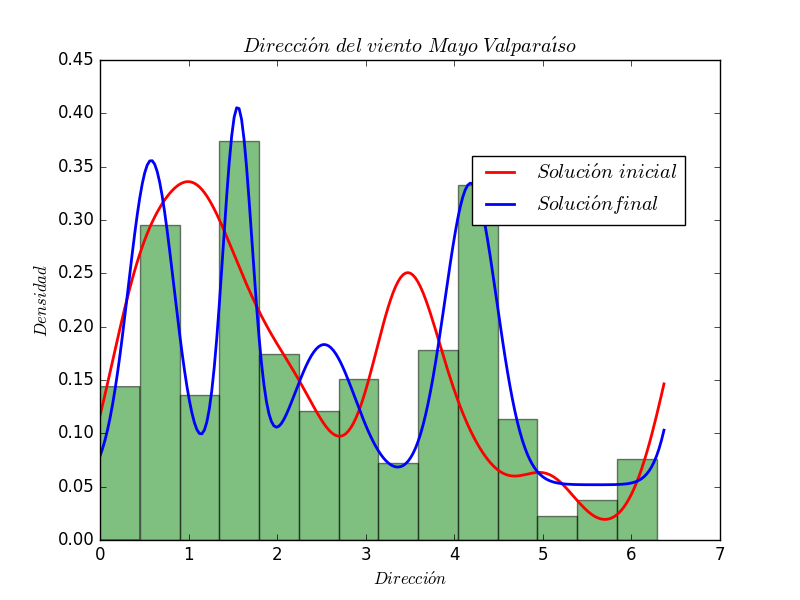
\includegraphics[width=0.42\textwidth]{figures/sol_ini_sol_fin_MAYO.png}
        }
         \subfigure[Solución inicial y final, Junio.]{
            \label{fig:PLOT_SOL_JUNIO}
            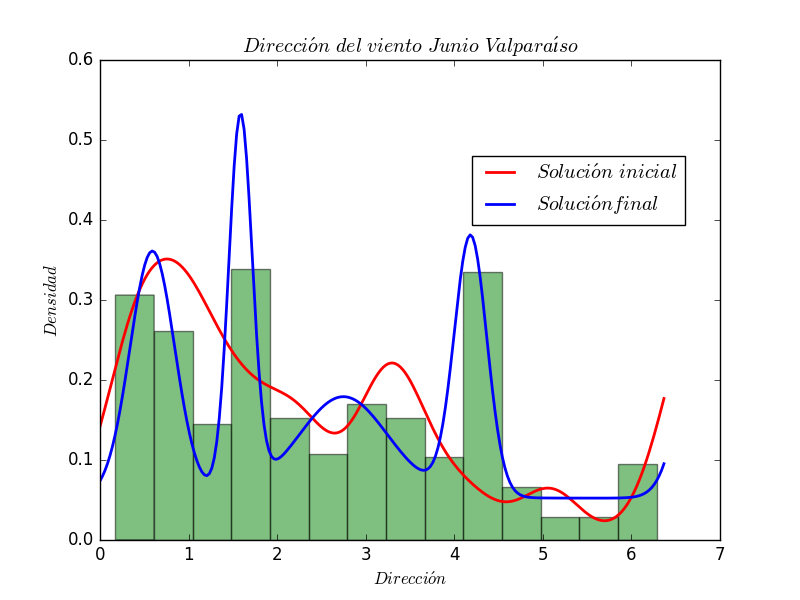
\includegraphics[width=0.42\textwidth]{figures/sol_ini_sol_fin_JUNIO.png}
        }
    \caption{Gráficos de ajuste de MVM por meses.}
    \caption*{Fuente: Elaboración propia.}
    \label{fig:PLOT_MONTHS_ALL_1}
\end{figure}
\newpage
\begin{figure}[ht!]
    \centering
    \captionsetup{justification=centering,margin=2cm}
        \subfigure[Solución inicial y final, Julio.]{
            \label{fig:PLOT_SOL_JULIO}
            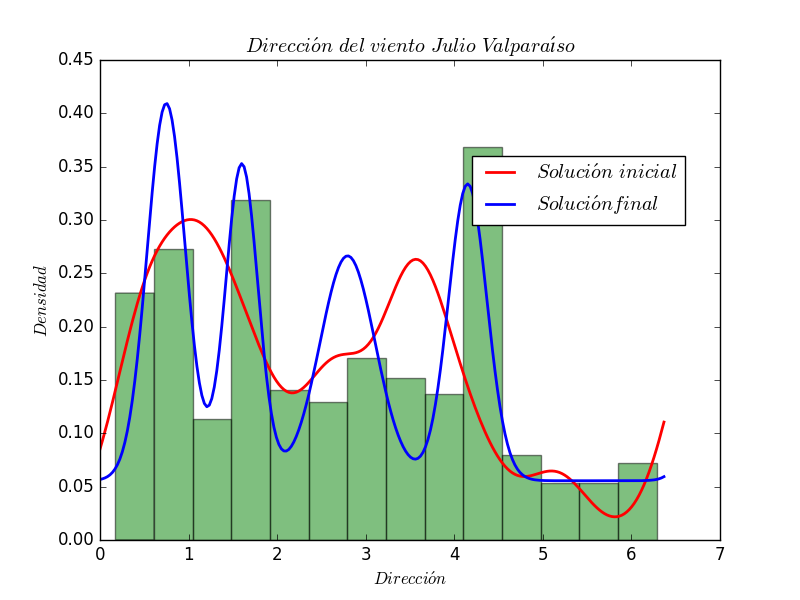
\includegraphics[width=0.42\textwidth]{figures/sol_ini_sol_fin_JULIO.png}
        }
         \subfigure[Solución inicial y final, Agosto.]{
            \label{fig:PLOT_SOL_AGOSTO}
            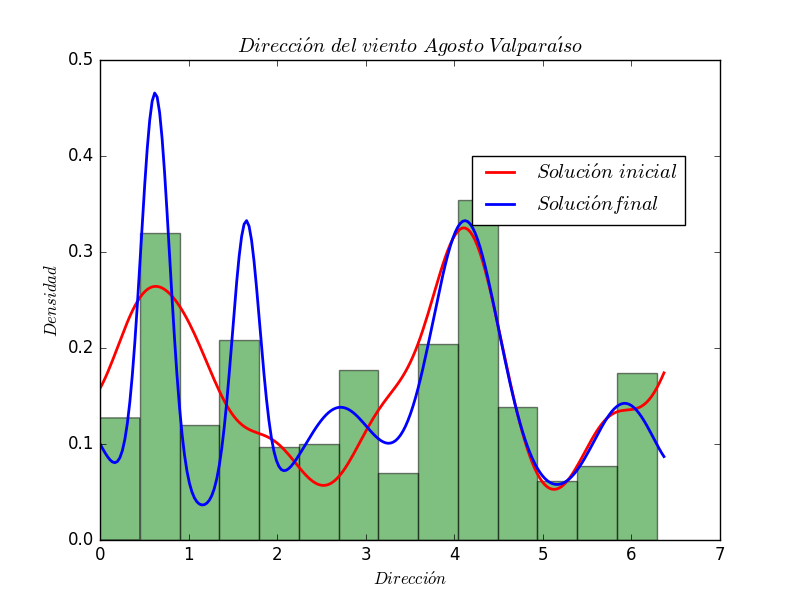
\includegraphics[width=0.42\textwidth]{figures/sol_ini_sol_fin_AGOSTO.png}
        }\\
          \subfigure[Solución inicial y final, Septiembre.]{
            \label{fig:PLOT_SOL_SEPTIEMBRE}
            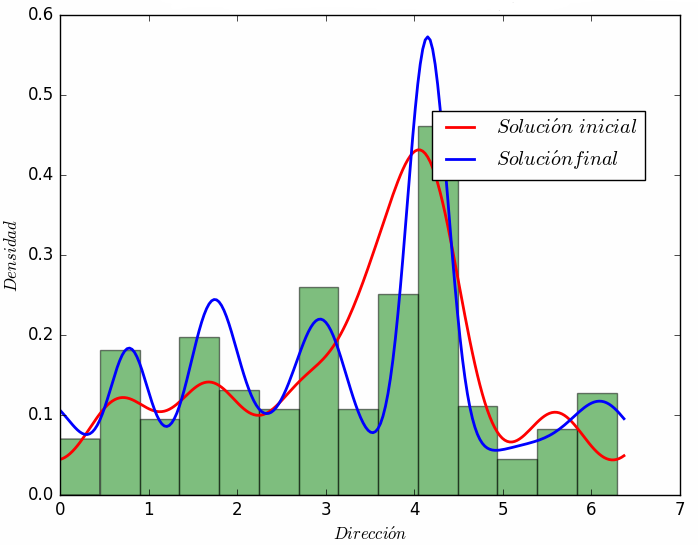
\includegraphics[width=0.42\textwidth]{figures/sol_ini_sol_fin_SEPTIEMBRE.png}
        }
         \subfigure[Solución inicial y final, Octubre.]{
            \label{fig:PLOT_SOL_OCTUBRE}
            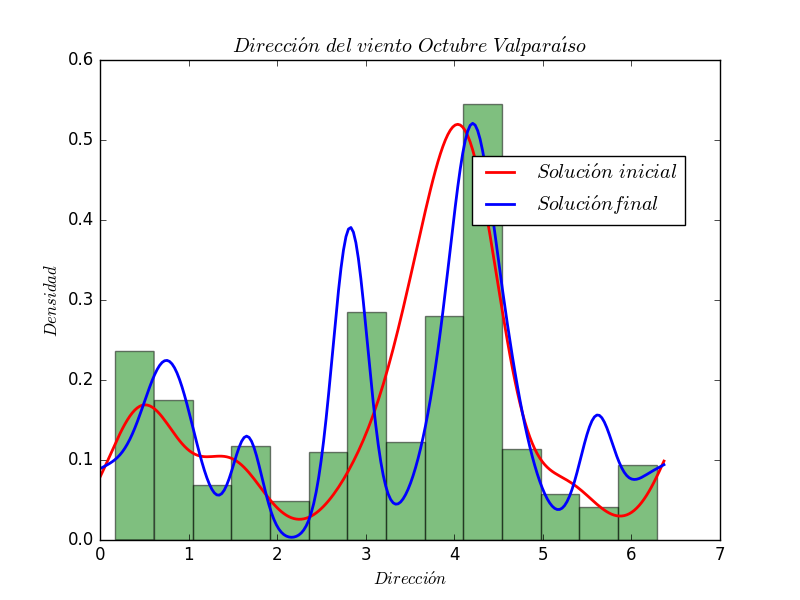
\includegraphics[width=0.42\textwidth]{figures/sol_ini_sol_fin_OCTUBRE.png}
        }\\
          \subfigure[Solución inicial y final, Noviembre.]{
            \label{fig:PLOT_SOL_NOVIEMBRE}
            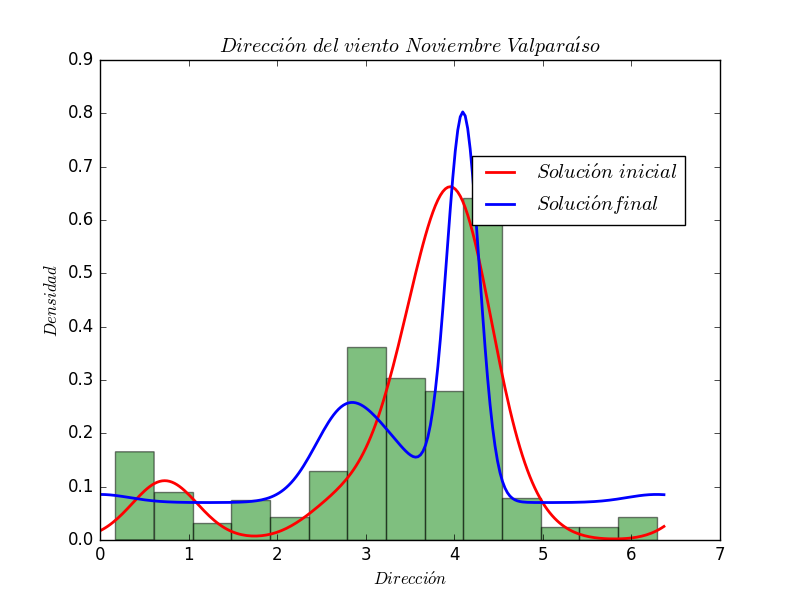
\includegraphics[width=0.42\textwidth]{figures/sol_ini_sol_fin_NOVIEMBRE.png}
        }
         \subfigure[Solución inicial y final, Diciembre.]{
            \label{fig:PLOT_SOL_DICIEMBRE}
            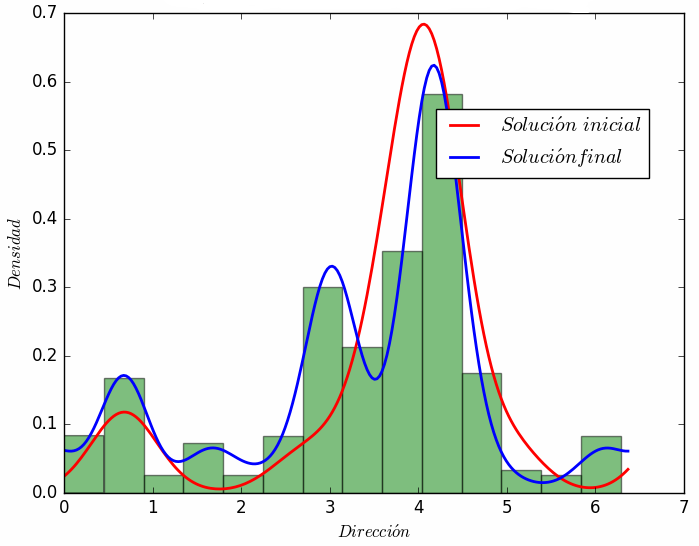
\includegraphics[width=0.42\textwidth]{figures/sol_ini_sol_fin_DICIEMBRE.png}
        }
    \caption{Gráficos de ajuste de MVM por meses.}
    \caption*{Fuente: Elaboración propia.}
    \label{fig:PLOT_MONTHS_ALL_2}
\end{figure}

\subsubsection{Experimento 4, Ajuste por meses, visualización en coordenadas polares}
En las Figuras agrupadas \ref{fig:PLOT_MONTHS_1} y \ref{fig:PLOT_MONTHS_2} se aprecia una visualización más interesante. Allí se puede ver de forma más intuitiva las direcciones dominantes del viento, relativas al sistema de referencia utilizado en meteorología conocido comúnmente como la rosa de los vientos \cite{RosaViento}. En el mes de Enero, Figuras \ref{fig:polar_ene_2015} \ref{fig:polar_ene_2014} \ref{fig:polar_ene_2013}, los vientos parecen provenir principalmente desde el suroeste, mientras que en Mayo, Figuras \ref{fig:polar_may_2015} \ref{fig:polar_may_2014} \ref{fig:polar_may_2013}, el origen del viento es más variable, proviniendo desde el noreste y el sur principalmente. En Septiembre, Figuras \ref{fig:polar_sep_2015} \ref{fig:polar_sep_2014} \ref{fig:polar_sep_2013}, vuelve a ser una fuente de los vientos predominante el suroeste.
\begin{figure}[ht!]
    \centering
    \captionsetup{justification=centering,margin=2cm}
        \subfigure[Dirección enero 2015.]{
            \label{fig:polar_ene_2015}
            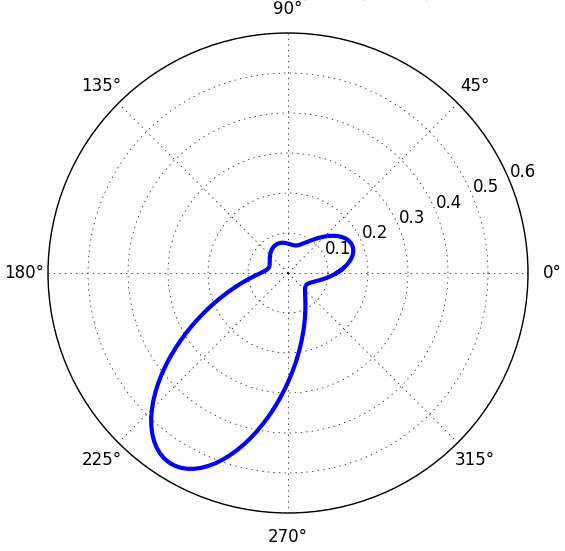
\includegraphics[width=0.43\textwidth]{figures/direction_enero_2015.png}
        }
         \subfigure[Dirección enero 2014.]{
            \label{fig:polar_ene_2014}
            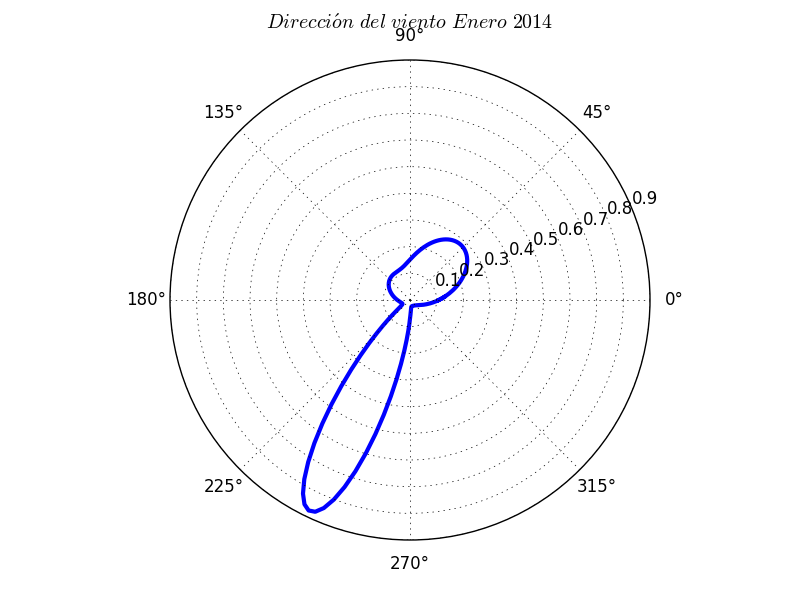
\includegraphics[width=0.43\textwidth]{figures/direction_enero_2014.png}
        }\\
         \subfigure[Dirección enero 2013.]{
            \label{fig:polar_ene_2013}
            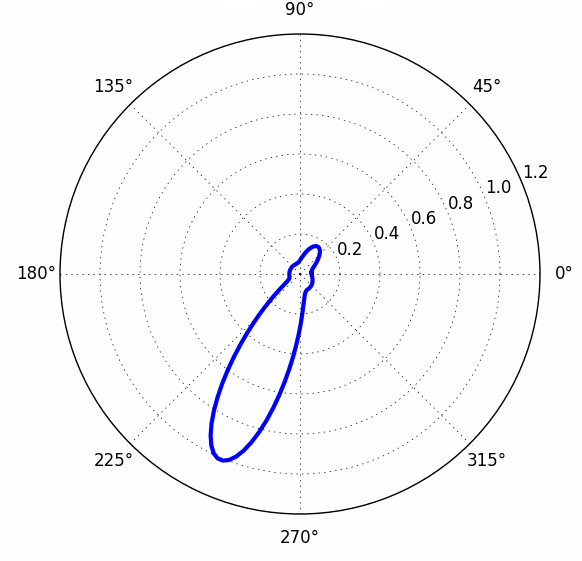
\includegraphics[width=0.43\textwidth]{figures/direction_enero_2013.png}
        }
         \subfigure[Dirección mayo 2015.]{
            \label{fig:polar_may_2015}
            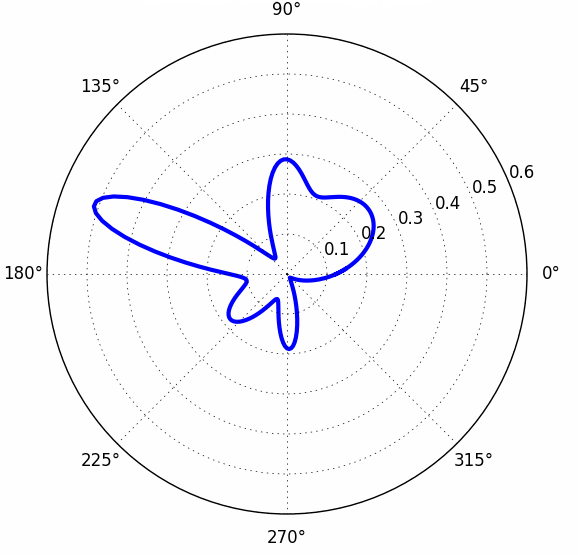
\includegraphics[width=0.43\textwidth]{figures/direction_mayo_2015.png}
        }\\
         \subfigure[Dirección mayo 2014.]{
            \label{fig:polar_may_2014}
            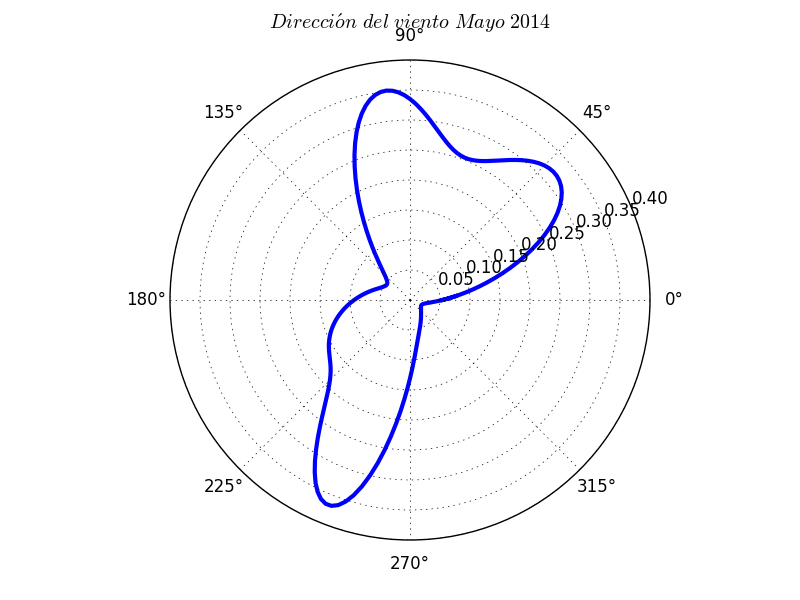
\includegraphics[width=0.43\textwidth]{figures/direction_mayo_2014.png}
        }
         \subfigure[Dirección mayo 2013.]{
            \label{fig:polar_may_2013}
            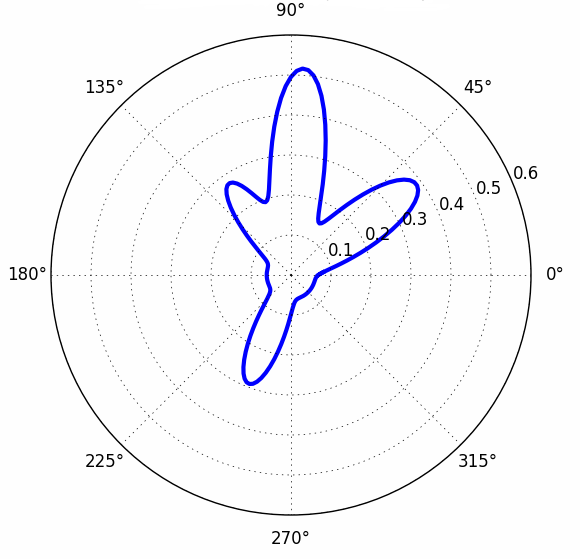
\includegraphics[width=0.43\textwidth]{figures/direction_mayo_2013.png}
        }
    \caption{Gráficos de ajuste por meses en coordenadas polares.}
    \caption*{Fuente: Elaboración propia.}
    \label{fig:PLOT_MONTHS_1}
\end{figure}

\begin{figure}[ht!]
    \centering
    \captionsetup{justification=centering,margin=2cm}
        \subfigure[Dirección septiembre 2015.]{
            \label{fig:polar_sep_2015}
            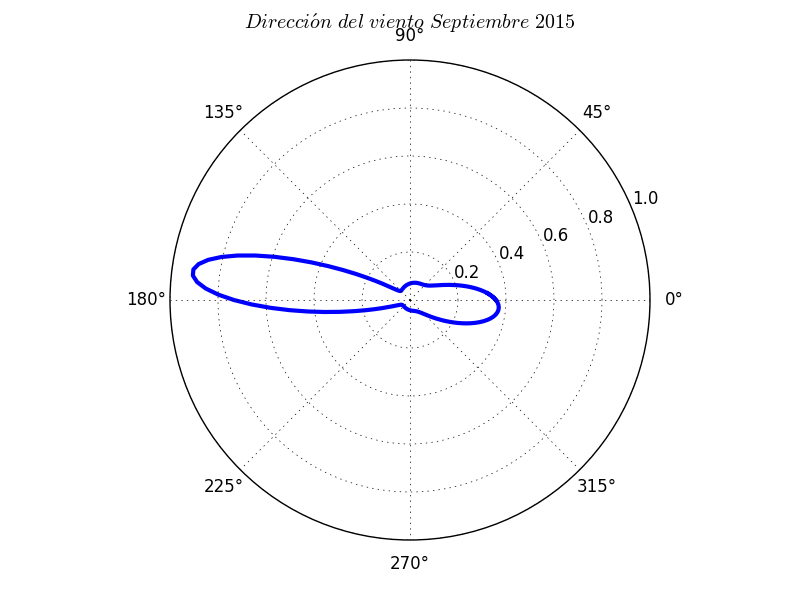
\includegraphics[width=0.45\textwidth]{figures/direction_septiembre_2015.png}
        }
         \subfigure[Dirección septiembre 2014.]{
            \label{fig:polar_sep_2014}
            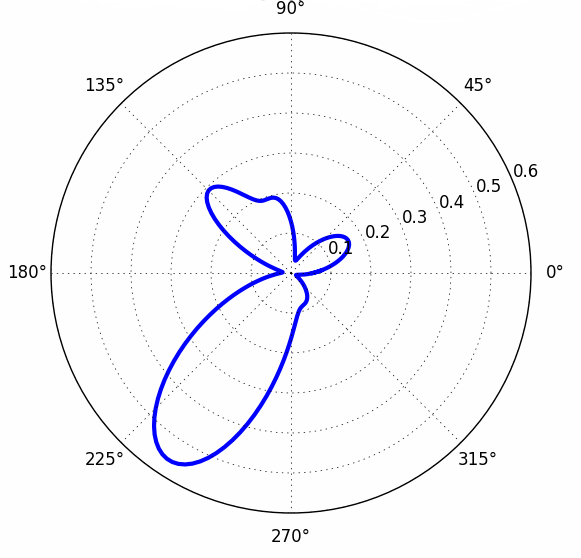
\includegraphics[width=0.45\textwidth]{figures/direction_septiembre_2014.png}
        }\\
         \subfigure[Dirección septiembre 2013.]{
            \label{fig:polar_sep_2013}
            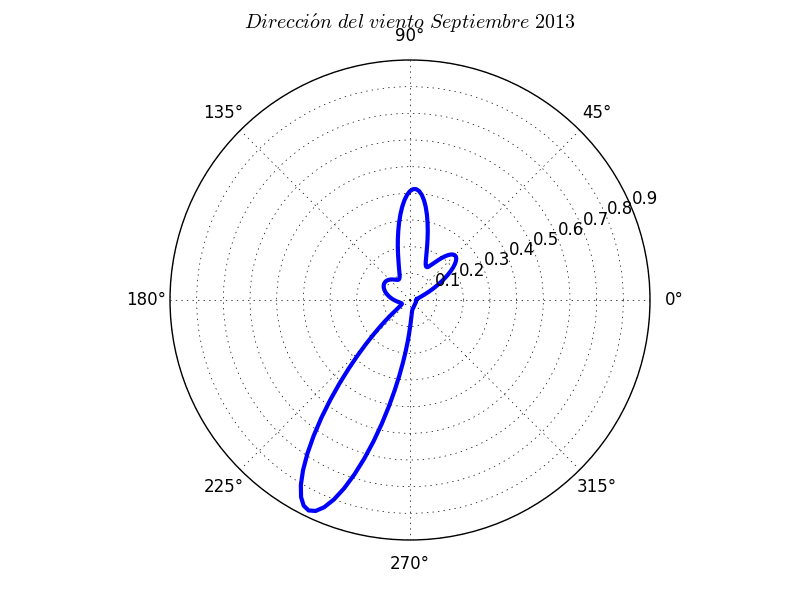
\includegraphics[width=0.45\textwidth]{figures/direction_septiembre_2013.png}
        }  
    \caption{Gráficos de ajuste por meses en coordenadas polares.}
    \caption*{Fuente: Elaboración propia.}
    \label{fig:PLOT_MONTHS_2}
\end{figure}

\subsubsection{Resumen de los experimentos}
%\begin{table}[ht!]
%    %\centering
%    \caption{Tabla de pruebas, PSO dirección del viento}
%    \label{table:stadistical_tests_direction}
%    \resizebox{\textwidth}{!}{
%    \begin{tabular}{|c|c|c|c|c|c|c|c|c|}
%        \hline
%        \textbf{Periodo de tiempo} & \textbf{PSI} & \textbf{PSFV} & \textbf{PSFF} & \textbf{Tiempo V} & \textbf{Tiempo F} & \textbf{Iteraciones V} & \textbf{%Iteraciones F} & \textbf{Cantidad datos}\\
%        \hline
%        2015            & 461,83    & -         & 251,37    & -           & 38m46,1s    & -     & 50500 & 2076 \\
%        2015            & 461,83    & 21,58     & 234,97    & 8m5,7s      & 47m47,1s    & 9005  & 50500 & 2076 \\
%        2014            & 301,12    & 24,86     & 56,57     & 20m37,8s    & 46m23,2s    & 29494 & 50500 & 2499 \\ 
%        2013            & 424,24    & 33,76     & 69,53     & 11m41,1s    & 48m23,7s    & 16778 & 50500 & 2346 \\
%        \hline
%        Enero           & 144,42    & 20,89     & 22,18     & 0m3,3s      & 25m37,2s    & 86    & 27276 & 633 \\
%        Febrero         & 130,39    & 19,45     & 22,27     & 0m12,2s     & 0m07,1s     & 288   & 134   & 567\\
%        Marzo           & 104,54    & 18,61     & 22,31     & 0m3,1s      & 0m13,3s     & 49    & 228   & 564 \\
%        Abril           & 74,97     & 21,13     & 22,25     & 0m12,5s     & 17m58,4s    & 192   & 18544 & 559 \\
%        Mayo            & 243,65    & 21,65     & 81,75     & 1m6,9s      & 42m59,6s    & 1237  & 50000 & 589 \\
%        Junio           & 286,30    & 21,01     & 188,91    & 1m42,9s     & 40m52,5s    & 1989  & 50000 & 554 \\
%        Julio           & 177,33    & 22,06     & 31,39     & 0m17,8s     & 45m48,3s    & 315   & 50000 & 604 \\
%        Agosto          & 79,57     & 21,94     & 22,17     & 0m12,9s     & 40m26,3s    & 202   & 41204 & 578 \\
%        Septiembre      & 92,77     & 21,31     & 22,31     & 0m1,7s      & 0m1,7s      & 27    & 166   & 541 \\
%        Octubre         & 188,14    & 21,81     & 37,50     & 0m45,3s     & 42m56,4s    & 825   & 50000 & 564 \\
%        Noviembre       & 363,90    & 26,25     & 88,16     & 42m21,4s    & 42m53,6s    & 50500 & 50000 & 582 \\
%        Diciembre       & 335,28    & 22,30     & 37,81     & 9m56,1s     & 43m52,9s    & 11640 & 50000 & 586 \\
%        \hline 
%        Enero 2015      & 42,94     & 16,34     & 18,77     & 0m4,1s      & 0m0,1s      & 61    & 10    & 220 \\
%        Enero 2014      & 68,10     & 20,68     & 21,61     & 0m1,8s      & 0m0,7s      & 29    & 126   & 206 \\
%        Enero 2013      & 194,98    & 19,31     & 24,86     & 0m0,4s      & 46m29,2s    & 6     & 50000 & 207 \\
%        Mayo 2015       & 60,84     & 17,99     & 26,69     & 0m2,3s      & 41m53,8s    & 39    & 50000 & 173 \\
%        Mayo 2014       & 142,85    & 20,94     & 20,48     & 0m4,8s      & 0m0,3s      & 82    & 50    & 213 \\
%        Mayo 2013       & 135,68    & 20,88     & 22,34     & 0m5,3s      & 0m1,1s      & 97    & 2089  & 203 \\
%        Septiembre 2015 & 77,41     & 21,29     & 25,54     & 0m8,4s      & 41m48,7s    & 137   & 50000 & 140 \\
%        Septiembre 2014 & 19,56     & 18,24     & 15,86     & 0m0,1s      & 0m0,1s      & 1     & 1     & 200 \\
%        Septiembre 2013 & 68,90     & 16,61     & 21,89     & 0m0,3s      & 0m0,9s      & 5     & 150   & 201 \\
%        \hline  
%    \end{tabular}
%    }   
%\end{table}

\begin{table}[ht!]
    %\centering
    \caption{Tabla de pruebas y repeticiones, PSO dirección del viento, Estrategia Variable}
    \label{table:repetitions_tests_direction_variable}
    \resizebox{\textwidth}{!}{
    \begin{tabular}{|c|c|c|c|c|c|c|c|c|c|c|c|}
        \hline
        \textbf{Periodo de tiempo} & \textbf{Puntaje Inicial} & \textbf{Menor Puntaje} & \textbf{Mayor Puntaje} & \textbf{Promedio Puntaje} & \textbf{Menor Iteraciones} & \textbf{Mayor Iteraciones} & \textbf{Promedio Iteraciones} & \textbf{Menor Tiempo} & \textbf{Mayor Tiempo} & \textbf{Promedio Tiempo} & \textbf{Cantidad datos}\\
        \hline
        2015            & 461,83    & 19,42     & 86,60  & 32,11 & 445   & 26395 & 13314 & 34   & 1800  &  992   & 2076 \\
        2014            & 301,12    & 17,08     & 59,73  & 36,18 & 4914  & 25904 & 22633 & 359  & 1800  &  1655  & 2499 \\ 
        2013            & 424,24    & 17,94     & 81,44  & 26,24 & 838   & 26048 & 12307 & 65   & 1800  &  925   & 2346 \\
        \hline  
        Enero           & 144,42    & 20,75     & 22,33  & 21,76 & 22    & 22515 & 1918  & 1    & 1558  & 136    & 633 \\
        Febrero         & 130,39    & 17,69     & 24,24  & 21,70 & 185   & 27321 & 3978  & 14   & 1800  & 277    & 567\\
        Marzo           & 104,54    & 16,90     & 24,38  & 21,57 & 37    & 25994 & 2448  & 3    & 1800  & 174    & 564 \\
        Abril           & 74,97     & 17,19     & 22,35  & 21,20 & 41    & 3369  & 589   & 3    & 235   & 42     & 559 \\
        Mayo            & 243,65    & 18,86     & 22,34  & 21,46 & 58    & 2281  & 559   & 4    & 166   & 41     & 589 \\
        Junio           & 286,30    & 20,36     & 22,35  & 21,98 & 50    & 2229  & 754   & 4    & 161   & 55     & 554 \\
        Julio           & 177,33    & 16,29     & 22,33  & 21,12 & 53    & 585   & 258   & 4    & 43    & 19     & 604 \\
        Agosto          & 79,57     & 16,42     & 22,30  & 20,99 & 12    & 2155  & 208   & 1    & 171   & 16     & 578 \\
        Septiembre      & 92,77     & 14,48     & 22,34  & 20,55 & 16    & 227   & 70    & 1    & 18    & 6      & 541 \\
        Octubre         & 188,14    & 19,21     & 24,41  & 21,89 & 300   & 25702 & 6607  & 22   & 1800  & 479    & 564 \\
        Noviembre       & 363,90    & 21,90     & 46,00  & 27,00 & 2288  & 25956 & 23969 & 168  & 1800  & 1725   & 582 \\
        Diciembre       & 335,28    & 21,55     & 64,28  & 27,68 & 5179  & 28004 & 20210 & 364  & 1800  & 1364   & 586 \\
        \hline 
        Enero 2015      & 42,94     & 18,68     & 22,33  & 20,50 & 3     & 81    & 29    & 1    & 6     &  2     & 220 \\
        Enero 2014      & 68,10     & 16,71     & 22,35  & 20,39 & 7     & 438   & 61    & 1    & 32    &  5     & 206 \\
        Enero 2013      & 194,98    & 15,41     & 22,30  & 19,98 & 10    & 245   & 76    & 1    & 19    &  6     & 207 \\
        Mayo 2015       & 60,84     & 17,68     & 22,28  & 20,97 & 5     & 107   & 38    & 1    & 8     &  3     & 173 \\
        Mayo 2014       & 142,85    & 16,30     & 22,30  & 20,22 & 9     & 52    & 24    & 1    & 4     &  2     & 213 \\
        Mayo 2013       & 135,68    & 15,16     & 21,99  & 19,86 & 2     & 159   & 24    & 1    & 13    &  2     & 203 \\
        Septiembre 2015 & 77,41     & 11,13     & 22,29  & 19,70 & 8     & 2529  & 690   & 1    & 219   &  60    & 140 \\
        Septiembre 2014 & 19,56     & 11,01     & 22,31  & 19,54 & 1     & 27    & 10    & 1    & 2     &  1     & 200 \\
        Septiembre 2013 & 68,90     & 12,29     & 22,33  & 19,92 & 10    & 175   & 35    & 1    & 12    &  3     & 201 \\
        \hline  
    \end{tabular}
    }   
\end{table}

\begin{table}[ht!]
    %\centering
    \caption{Tabla de pruebas y repeticiones, PSO dirección del viento, Estrategia Fija}
    \label{table:repetitions_tests_direction_fijo}
    \resizebox{\textwidth}{!}{
    \begin{tabular}{|c|c|c|c|c|c|c|c|c|c|c|c|}
        \hline
        \textbf{Periodo de tiempo} & \textbf{Puntaje Inicial} & \textbf{Menor Puntaje} & \textbf{Mayor Puntaje} & \textbf{Promedio Puntaje} & \textbf{Menor Iteraciones} & \textbf{Mayor Iteraciones} & \textbf{Promedio Iteraciones} & \textbf{Menor Tiempo} & \textbf{Mayor Tiempo} & \textbf{Promedio Tiempo} & \textbf{Cantidad datos}\\
        \hline
        2015            & 461,83    & 51,79     & 380,40  & 137,07 & 24082  & 27506 & 25651 & 1800 & 1800  & 1800  & 2076 \\
        2014            & 301,12    & 62,07     & 314,62  & 122,52 & 21681  & 26393 & 24633 & 1800 & 1800  & 1800  & 2499 \\
        2013            & 424,24    & 65,76     & 433,80  & 182,85 & 21684  & 27603 & 23866 & 1800 & 1800  & 1800  & 2346 \\
        \hline  
        Enero           & 144,42    & 22,30     & 96,99   & 49,17 & 940     & 26675 & 23210 & 68   & 1800  & 1699  & 633 \\
        Febrero         & 130,39    & 23,20     & 87,79   & 46,30 & 22926   & 26619 & 24898 & 1800 & 1800  & 1800  & 567\\
        Marzo           & 104,54    & 21,15     & 106,97  & 45,49 & 376     & 26552 & 22377 & 28   & 1800  & 1647  & 564 \\
        Abril           & 74,97     & 19,82     & 84,00   & 33,61 & 54      & 27723 & 13408 & 5    & 1800  & 948   & 559 \\
        Mayo            & 243,65    & 21,98     & 52,87   & 28,44 & 212     & 25973 & 20789 & 16   & 1800  & 1519  & 589 \\
        Junio           & 286,30    & 22,76     & 188,91  & 50,13 & 20320   & 27830 & 23479 & 1668 & 1800  & 1756  & 554 \\
        Julio           & 177,33    & 23,05     & 72,56   & 33,93 & 127     & 26587 & 21869 & 55   & 1800  & 1533  & 604 \\
        Agosto          & 79,57     & 20,45     & 78,96   & 25,72 & 66      & 25514 & 19256 & 7    & 1800  & 1623  & 578 \\
        Septiembre      & 92,77     & 21,30     & 64,74   & 32,17 & 155     & 27258 & 20122 & 47   & 1800  & 1414  & 541 \\
        Octubre         & 188,14    & 22,35     & 102,38  & 38,70 & 277     & 26231 & 24109 & 36   & 1800  & 1563  & 564 \\
        Noviembre       & 363,90    & 32,69     & 150,89  & 63,91 & 359     & 26032 & 22324 & 20   & 1800  & 1899  & 582 \\
        Diciembre       & 335,28    & 24,35     & 90,86   & 47,12 & 15720   & 27111 & 21662 & 89   & 1800  & 1657  & 586 \\
        \hline 
        Enero 2015      & 42,94     & 15,24     & 38,07   & 22,51 & 17      & 27010  & 8265  & 1   & 1800   & 586  & 220 \\
        Enero 2014      & 68,10     & 17,16     & 32,71   & 21,78 & 11      & 26014  & 7265  & 1   & 1800   & 750  & 206 \\
        Enero 2013      & 194,98    & 14,58     & 41,95   & 30,89 & 6       & 25341  & 6541  & 1   & 1800   & 789  & 207 \\
        Mayo 2015       & 60,84     & 16,92     & 35,77   & 25,72 & 21      & 20147  & 7566  & 1   & 1800   & 852  & 173 \\
        Mayo 2014       & 142,85    & 19,32     & 56,89   & 30,88 & 62      & 24612  & 7894  & 3   & 1800   & 421  & 213 \\
        Mayo 2013       & 135,68    & 18,26     & 46,33   & 33,90 & 44      & 20144  & 8742  & 1   & 1800   & 520  & 203 \\
        Septiembre 2015 & 77,41     & 19,52     & 30,45   & 21,14 & 79      & 24700  & 8440  & 2   & 1800   & 324  & 140 \\
        Septiembre 2014 & 19,56     & 14,36     & 29,51   & 24,55 & 1       & 20892  & 3247  & 1   & 1800   & 385  & 200 \\
        Septiembre 2013 & 68,90     & 16,86     & 32,48   & 22,63 & 5       & 24113  & 4570  & 1   & 1800   & 480  & 201 \\
        \hline  
    \end{tabular}
    }   
\end{table}

\begin{figure}[ht!]
    \centering
    \captionsetup{justification=centering,margin=2cm}
        \subfigure[Puntajes obtenidos con la estrategia Variable.]{
            \label{fig:polar_ene_2015}
            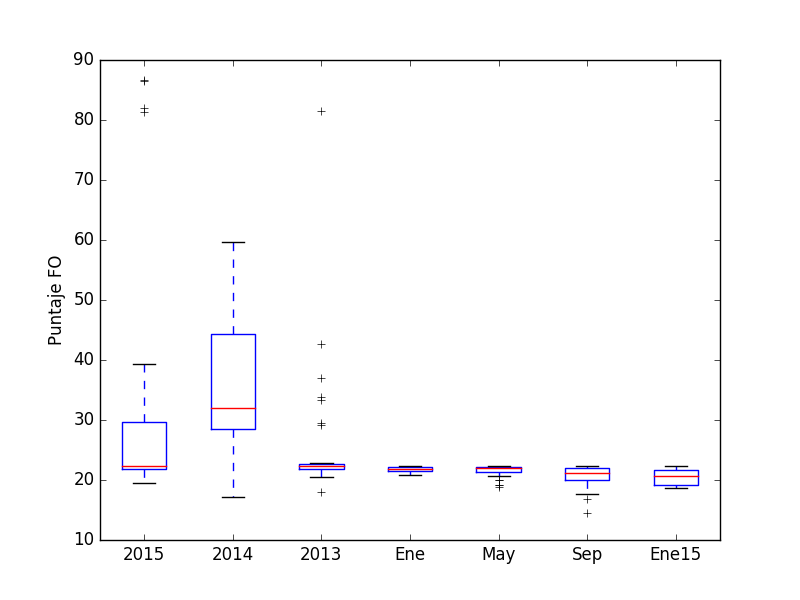
\includegraphics[width=0.45\textwidth]{figures/bp_puntaje_V.png}
        }
         \subfigure[Puntajes obtenidos con la estrategia Fija.]{
            \label{fig:polar_ene_2014}
            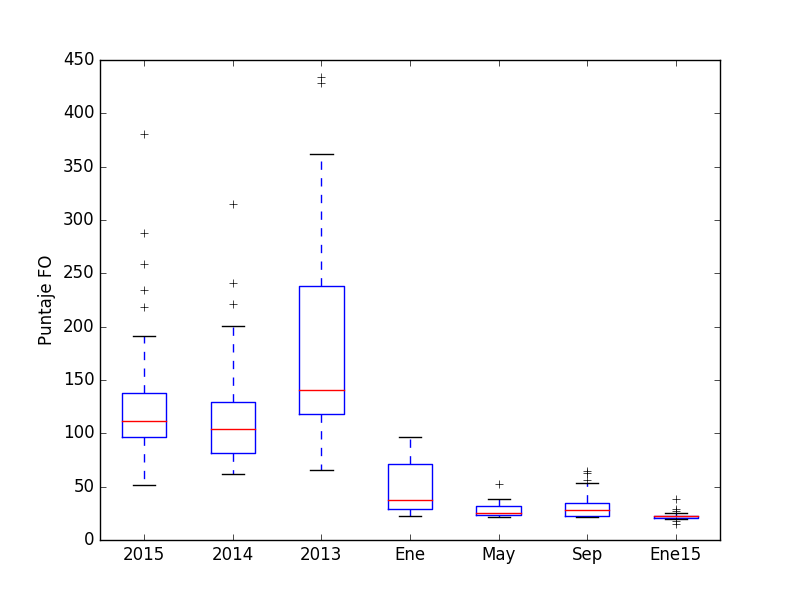
\includegraphics[width=0.45\textwidth]{figures/bp_puntaje_F.png}
        }\\
         \subfigure[Iteraciones alcanzadas con la estrategia Variable.]{
            \label{fig:polar_ene_2013}
            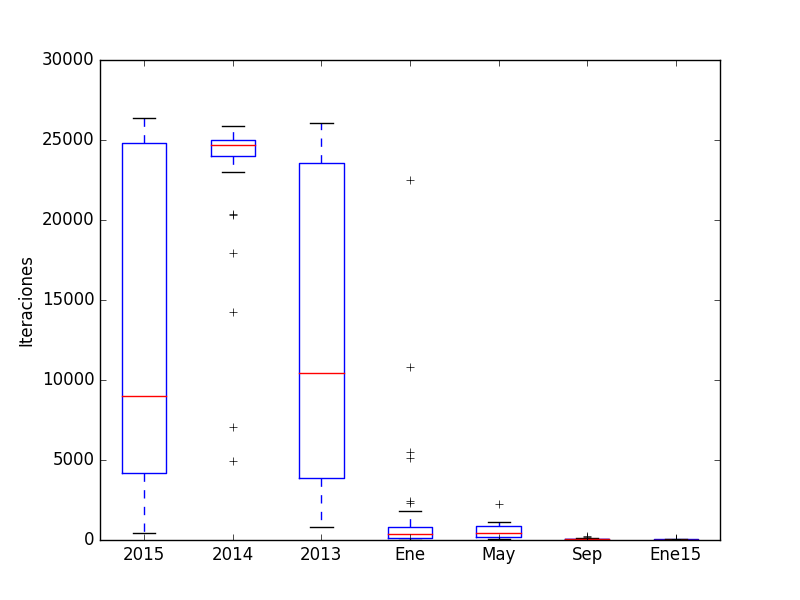
\includegraphics[width=0.45\textwidth]{figures/bp_iteraciones_V.png}
        }
         \subfigure[Iteraciones alcanzadas con la estrategia Fija.]{
            \label{fig:polar_may_2015}
            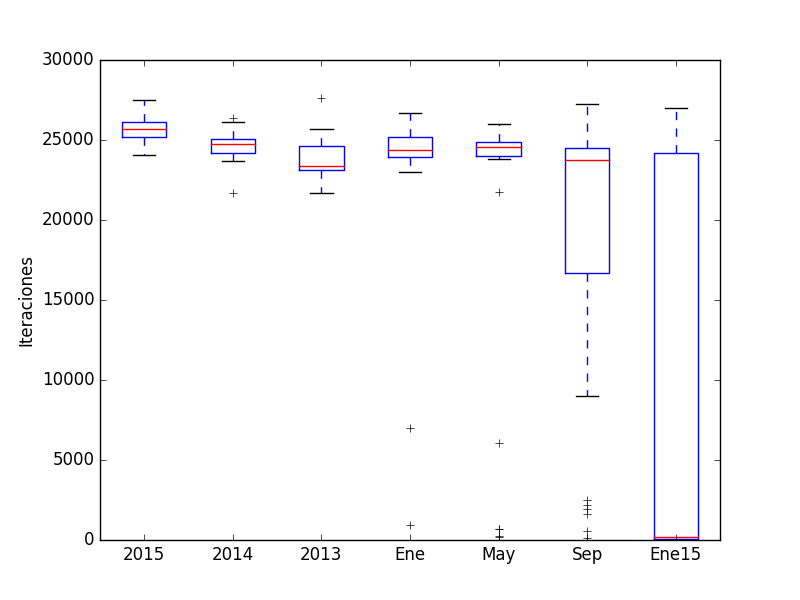
\includegraphics[width=0.45\textwidth]{figures/bp_iteraciones_F.png}
        }\\
         \subfigure[Tiempos empleado con la estrategia Variable.]{
            \label{fig:polar_may_2014}
            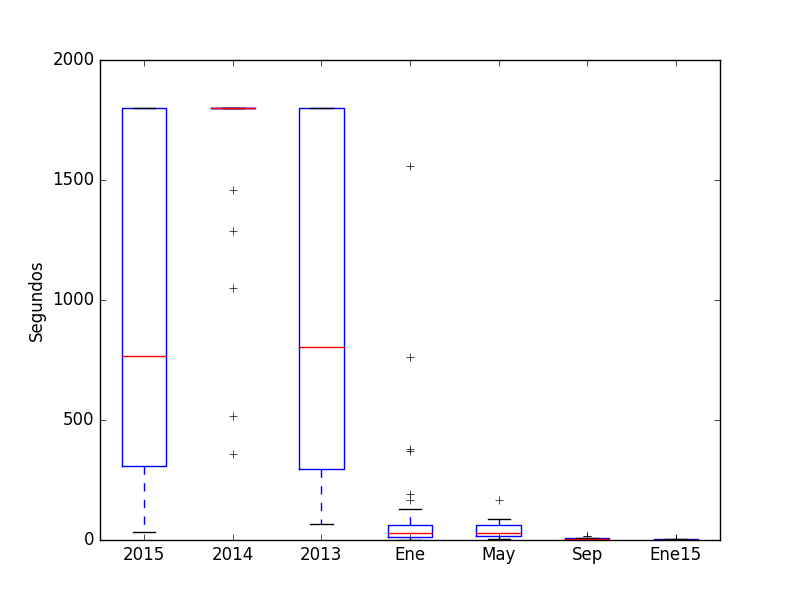
\includegraphics[width=0.45\textwidth]{figures/bp_tiempo_V.png}
        }
         \subfigure[Tiempos empleado con la estrategia Fija.]{
            \label{fig:polar_may_2013}
            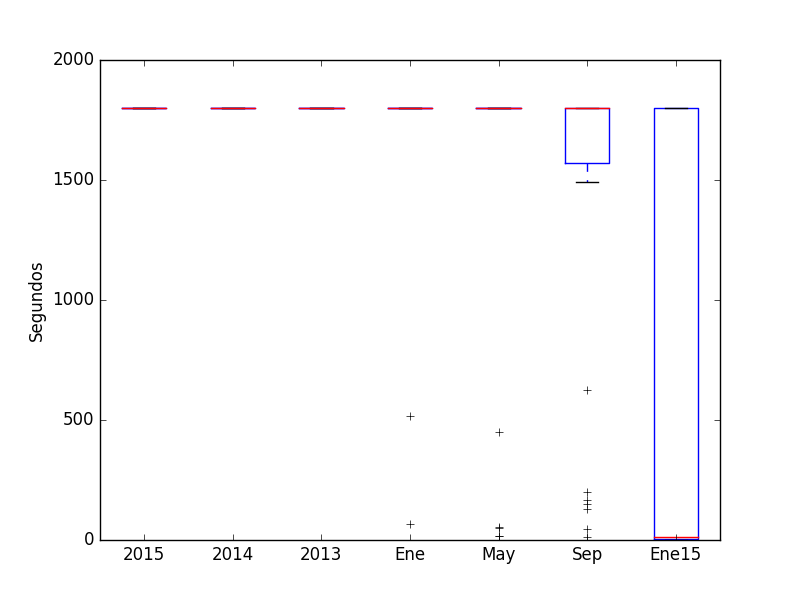
\includegraphics[width=0.45\textwidth]{figures/bp_tiempo_F.png}
        }
    \caption{Boxplots de repeticiones del PSO con al estratégia Fija y Variable.}
    \caption*{Fuente: Elaboración propia.}
    \label{fig:BOXPLOTS_DIRECTION}
\end{figure}


Las tablas \ref{table:repetitions_tests_direction_variable} y \ref{table:repetitions_tests_direction_fijo} muestran un resumen de los resultados obtenidos al ajustar la distribución de probabilidad \emph{von Mises distribution} en diferentes subconjuntos de tiempo de los datos colectados en los años 2013, 2014 y 2015, siguiendo la estrategia Variable (propuesta en esta memoria) y la estrategia Fija (sin variación de parámetros). Las tablas están organizadas como sigue a continuación. La estrategia \textbf{Variable} hace referencia a la propuesta realizada en esta memoria para la variación de parámetros del PSO explicada en la sección \ref{subsec:parametros_new}, mientras que la estrategia \textbf{Fijo} es la seguida en el trabajo de Heckenbergerova et al. \cite{Heckenbergerova15}, la cual consta de la definición de parámetros fijos para el PSO.
\begin{enumerate}
    \item \emph{Periodo de tiempo}: Rango de tiempo donde se consideraron los datos para el ajuste.
    \item \emph{Puntaje Inicial}: Puntaje solución inicial, es decir, el valor obtenido al evaluar la solución inicial en la función objetivo.
    \item \emph{Menor Puntaje}: Equivale al mejor puntaje obtenido por las repeticiones.
    \item \emph{Mayor Puntaje}: Equivale al peor puntaje obtenido por las repeticiones.
    \item \emph{Promedio Puntaje}: Puntaje promedio de las repeticiones.
    \item \emph{Menor Iteraciones}: Equivale a la mejor cantidad de iteraciones obtenidas por las repeticiones.
    \item \emph{Mayor Iteraciones}: Equivale a la mejor cantidad de iteraciones obtenidas por las repeticiones. 
    \item \emph{Promedio Iteraciones}: Iteraciones promedio de las repeticiones. 
    \item \emph{Menor Tiempo}: Equivale al mejor tiempo obtenido por las repeticiones.
    \item \emph{Mayor Tiempo}: Equivale al peor tiempo obtenido por las repeticiones.
    \item \emph{Promedio Tiempo}: Tiempo promedio de las repeticiones.
    \item \emph{Cantidad datos}: Cantidad de datos utilizados en el ajuste.
\end{enumerate}

\begin{figure}[ht!]
    \centering
    \captionsetup{justification=centering,margin=2cm}
        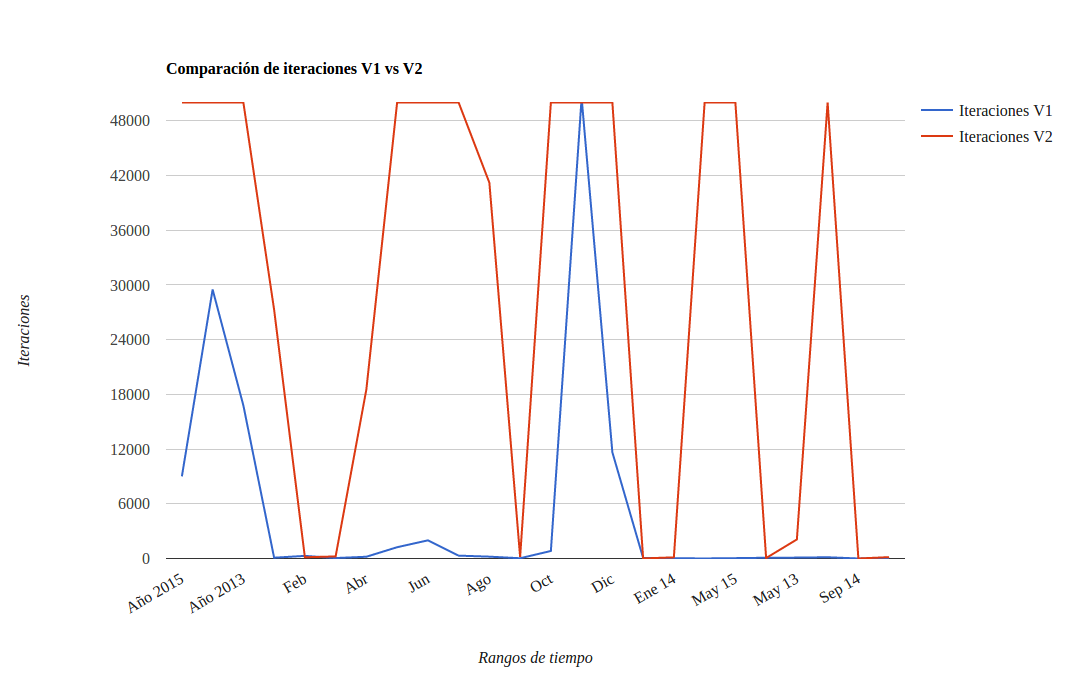
\includegraphics[width=\textwidth]{figures/comp_v1_v2_iteraciones.png}
        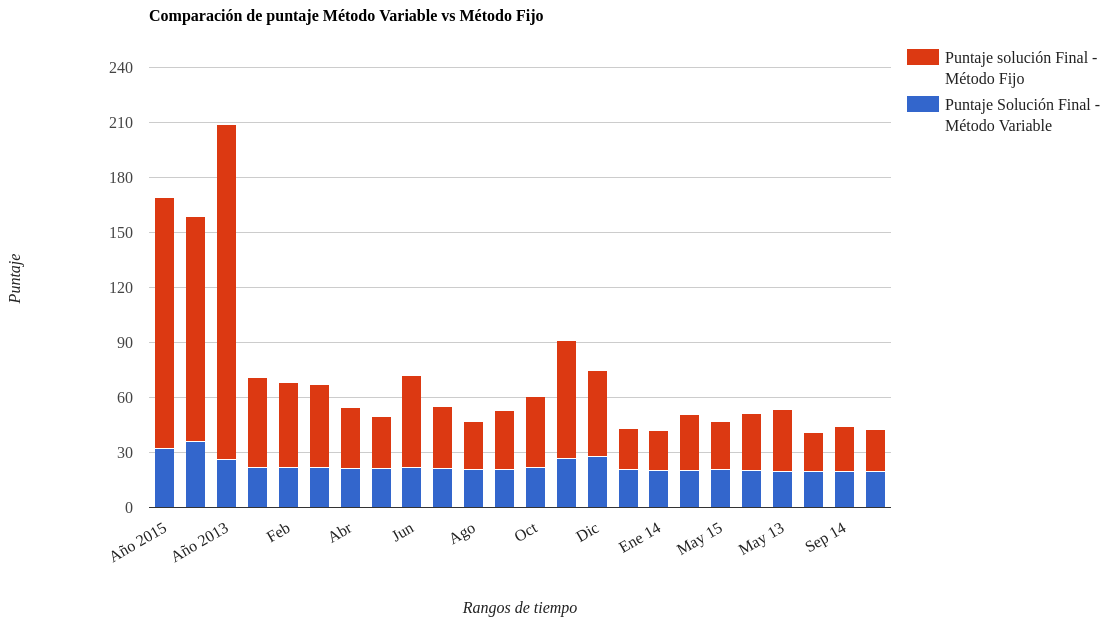
\includegraphics[width=\textwidth]{figures/comp_v1_v2_puntaje.png} 
    \caption{Comparación de variaciones en el PSO.}
    \caption*{Fuente: Elaboración propia.}
    \label{fig:comparison_pso_1}
\end{figure}

\begin{figure}[ht!]
    \centering
    \captionsetup{justification=centering,margin=2cm}
        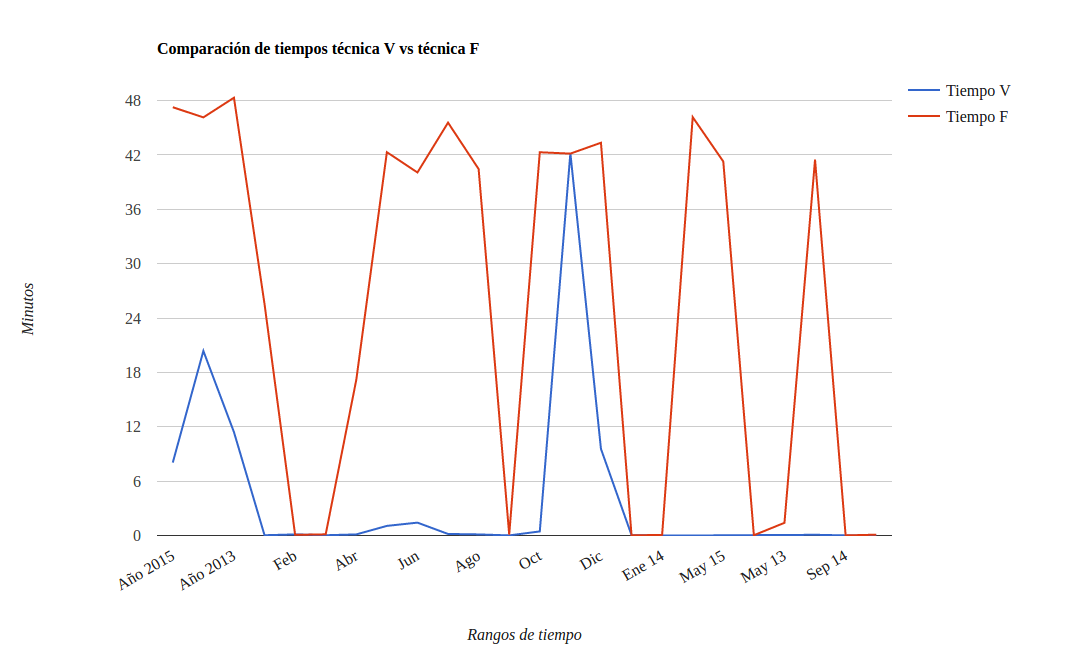
\includegraphics[width=\textwidth]{figures/comp_v1_v2_tiempo.png}   
    \caption{Comparación de variaciones en el PSO.}
    \caption*{Fuente: Elaboración propia.}
    \label{fig:comparison_pso_2}
\end{figure}
Los gráficos en \ref{fig:comparison_pso_1} y  \ref{fig:comparison_pso_2} muestran la comparación de los rendimientos de los algoritmos con parámetros fijos y variables para el PSO según la propuesta explicada en la sección \ref{subsec:parametros_new}. Es claro que en la mayoría de los experimentos, la propuesta realizada tiene mejor rendimiento y en el peor de los casos se comporta igual o levemente peor que la forma tradicional de parámetros fijos utilizada en el trabajo de Heckenbergerova et al. \cite{Heckenbergerova15}.\\
En las Figuras en \ref{fig:BOXPLOTS_DIRECTION}, se pueden observar la distribución de resultados para los puntajes, iteraciones y tiempos obtenidos por las repeticiones de algunos de los experimentos. En general los valores alcanzados son similares independiente de la semilla generadora de números aleatorios, a excepción de algunos casos particulares en donde se observa una alta dispersión, sobre todo en los experimentos del PSO con estrategia Fija.
\newpage
\section{Conclusiones del capítulo}
En este capítulo se ajustaron los parámetros de la función \emph{mixture of von Mises distribution} a datos de dirección del viento en Valparaíso. Basado en el trabajo de Heckenbergerova et al. \cite{Heckenbergerova15}, se implementó el \emph{Particle Swarm Optimization} con una modificación propuesta en esta memoria para mejorar los resultados del trabajo citado.\\
Como se puede ver en la tabla \ref{table:stadistical_tests_direction}, la modificación propuesta y explicada en las ecuaciones \ref{eq:VariationParameters_new}, \ref{eq:VariationParameters_new_2} y \ref{eq:VariationParameters_new_3} para el control de los parámetros del PSO, permite obtener mejores tiempos de ejecución y soluciones de mejor calidad que los valores utilizados en el trabajo de Heckenbergerova et al. \cite{Heckenbergerova15}. Esto se debe al problema de convergencia prematura del PSO, el cual no fue considerado en dicho trabajo. \\
De las Figuras expuestas en \ref{fig:PLOT_MONTHS_ALL_1} y \ref{fig:PLOT_MONTHS_ALL_2} se puede observar que a pesar del buen puntaje conseguido por la solución, el gráfico difiere del histograma en varias pruebas más de lo deseado. Esto se debe a que la función objetivo definida en el PSO procura que las áreas bajo la curva de la función de densidad de probabilidad coincidan con las del histograma, sin embargo, más de una forma de la función de densidad puede cumplir dicho objetivo. Para evitar este problema se podría modificar la función objetivo añadiendo una penalización a la distancia de los puntos de la curva con respecto a la altura de la sección del histograma correspondiente.\\
Finalmente, al variar la semilla de números aleatorios, se observa una mayor dispersión en los resultados obtenidos del PSO con la estrategia Fija (sin variar los parámetros del algoritmo durante la ejecución) en comparación con la propuesta realizada en esta memoria.